% --------------------------------------------------------------------------------------------------
% Section: Etiological Risk Factors
% This section introduces and outlines the primary causes and contributing factors behind lung 
% cancer, supported by global epidemiological context and risk exposure types.
% --------------------------------------------------------------------------------------------------

\section{Etiological Risk Factors}

% General overview of lung cancer's global burden and major risk contributors, including tobacco, 
% second-hand smoke, radon, occupational and environmental hazards, and newer factors.
Lung cancer is the leading cause of global cancer incidence and mortality. Tobacco smoking is the 
greatest preventable cause of death worldwide, accounting for up to 90\% of lung cancer cases, and 
continued consumption is projected to increase global cancer incidence, particularly in developing 
nations such as China, Russia, and India. Second-hand smoke among children and spouses has likewise 
been implicated. Radon from natural underground uranium decay is the second leading cause of lung 
cancer in the developed world. Occupational hazards such as asbestos and environmental exposures 
such as air pollution, arsenic, and HIV and Tb infection have all been implicated in lung 
carcinogenesis, while cannabis smoking, electronic cigarettes, heated tobacco products, and COVID-19 
have been hypothesized to increase risk. \cite{PMC8063897}

% Figure: Visual summary of major lung cancer risk factors
\vspace{1em}
\begin{center} 
    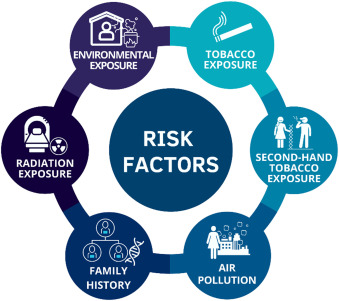
\includegraphics[width = 10cm, height = 9cm]{../assets/02-etiology/risk-factors-lunf-cancer.jpg}

    \small\textit{Risk factors for lung cancer. \cite{florez2023lung}}
\end{center}
\vspace{1em}

% --------------------------------------------------------------------------------------------------
% Subsection: Tobacco Use and Exposure
% Traces the historical correlation and mechanisms linking tobacco with lung cancer.
% --------------------------------------------------------------------------------------------------

\subsection{Tobacco Use and Exposure}

% Historical context: Correlation between rise in lung cancer and tobacco use in the early 20th century.
While, at the beginning of the twentieth century, lung cancer was a rare disease, it was diagnosed 
progressively more often over the next 50 years, and various suggestions were made during this 
period that cigarette smoking might be the cause, deriving mainly from the simple fact that the 
incidence and cigarette consumption were increasing concomitantly.\cite{Lee17} 

% Overview of tobacco's chemical composition and global impact on mortality.
Tobacco smoke is a complex chemical mixture, containing several thousand compounds, including at 
least 60 known carcinogens. It is reported that there are an estimated 1.1 billion smokers globally, 
1.8 million deaths from lung cancer each year, and about 80–90\% of those deaths are attributable to 
tobacco smoke exposure. \cite{JOUR}

% Figure: Global data on tobacco-related cancer mortality by country.
\vspace{1em}
\begin{center} 
    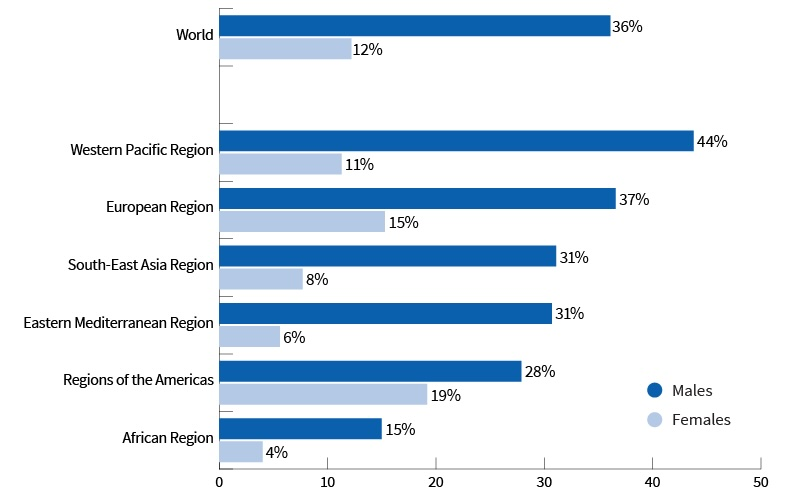
\includegraphics[width=\textwidth]{../assets/02-etiology/table-tobacco-use-by-country copy.jpg}

    \small\textit{Deaths from Cancer Caused from Using Tobacco, Worldwide in 2019. \cite{sandy2021}}
\end{center}
\vspace{1em} 

% Molecular mechanisms of carcinogenesis due to tobacco smoke.
% Covers DNA adduct formation, oxidative stress, disrupted repair pathways, and epigenetic changes.
There are several ways in which smoking promotes cancer. The primary method is harming our cells' 
DNA. Our cells' growth and behavior are governed by their DNA. Benzoapyrene and nitrosamines, two 
carcinogenic substances found in tobacco smoke, are the main source of DNA damage because they are 
metabolically converted into reactive intermediates in the body. By directly binding to DNA, these 
intermediates create chemical lesions known as DNA adducts, which alter the structure of DNA and 
obstruct proper transcription and replication. High amounts of reactive oxygen species (ROS) 
produced by tobacco smoking also cause oxidative stress, which harms DNA bases. Tobacco smoke not 
only directly damages DNA but also disrupts essential DNA repair processes such as base excision 
repair and nucleotide excision repair, which permits mutations to accumulate. Tobacco smoke also 
causes epigenetic modifications, like aberrant DNA methylation, which inhibit tumor suppressor 
genes and accelerate the development of cancer. All of these processes work together to explain the 
molecular link between cigarette smoke and lung cancer.

% --------------------------------------------------------------------------------------------------
% Subsection: Environmental and Air Pollutants
% Describes both outdoor and indoor air pollution as risk factors for lung cancer.
% --------------------------------------------------------------------------------------------------

\subsection{Environmental and Air Pollutants}

% Introduction to the impact of pollutants on lung cancer via carcinogenic and inflammatory pathways.
Environmental and air pollutants significantly influence lung cancer risk through both direct 
carcinogenic effects and chronic inflammatory mechanisms. The relationship varies by pollutant 
type, exposure duration, and geographic context, with outdoor and indoor sources contributing 
differently across income levels.

% Figure: Attribution of lung cancer deaths to air pollution (2021 data).
\vspace{1em}
\begin{center} 
    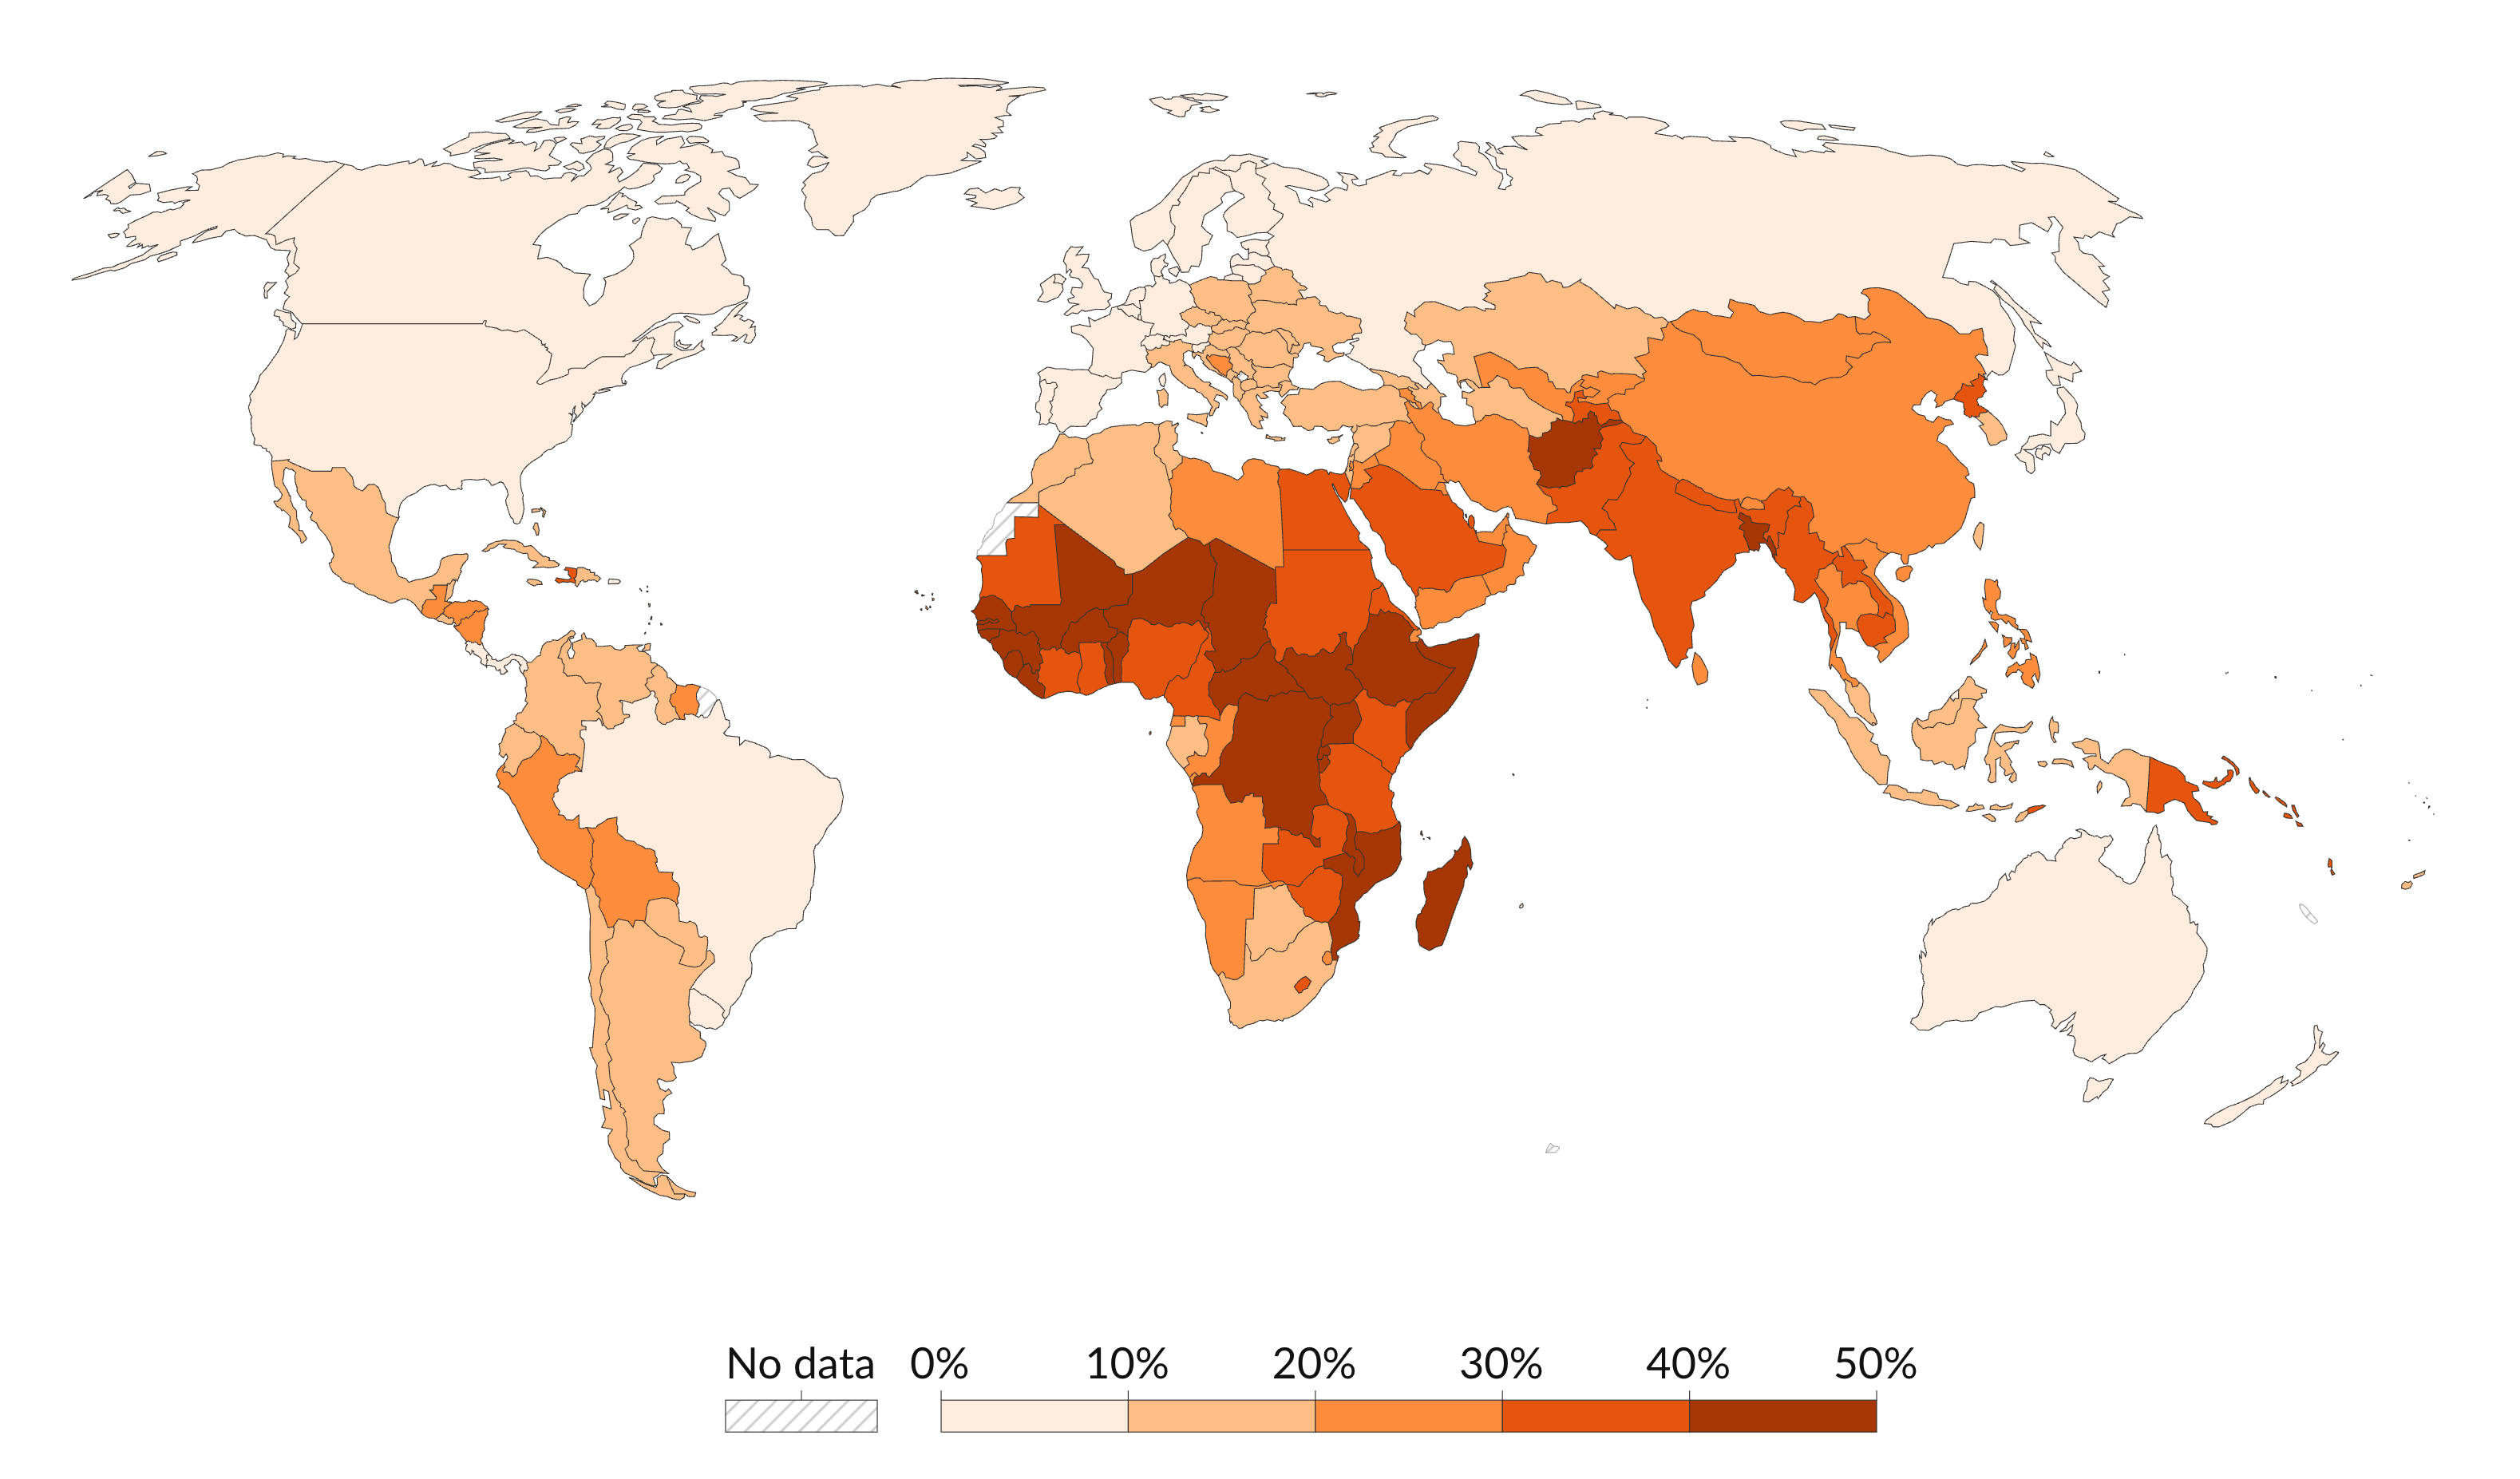
\includegraphics[width=\textwidth]{../assets/02-etiology/share-of-lung-cancer-deaths-attributed-to-air-pollution.png}

    \small\textit{The estimated share of lung cancer deaths attributed to the risk factor air 
    pollution, 2021. \cite{ihme2016}}
\end{center}
\vspace{1em} 

% Itemized breakdown of pollution types and regional effects.
\begin{itemize}
    \item \textbf{Outdoor Air Pollution:} Particulate matter is a major driver, with studies showing 
    a 10 $\mu$g/m³ increase in PM2.5 correlates with an 8\% rise in lung cancer mortality \cite{38513187} 
    and long-term exposure increases lung adenocarcinoma risk, particularly in urbanized areas. 
    Nitrogen dioxide (NO2) and ozone (O3) also contribute, with NO2 linked to a 3\% higher incidence 
    per 1\% concentration increase. Geographically, middle-income countries see a 0.28\% lung cancer 
    risk increase per 1\% rise in outdoor pollution, while high-income countries face a 0.51\% 
    increase. \cite{jco2023}

    \item \textbf{Indoor Air Pollution:} Sources like cooking fumes, coal burning, and radon 
    disproportionately affect high-income countries: a 1\% increase in indoor pollution raises lung 
    cancer risk by 0.37\% in these regions. \cite{fpubh.2024.1372320}
\end{itemize}

% Suggestion: Mitigation strategies for air pollution to reduce cancer incidence.
Lung cancer incidence might be significantly decreased by mitigating air pollution through stronger 
emission restrictions and the use of clean energy, especially in areas with quickly industrializing 
economies.

% --------------------------------------------------------------------------------------------------
% Subsection: Genetic and Familial Predisposition
% Describes inherited genetic mutations and familial aggregation of lung cancer risk.
% --------------------------------------------------------------------------------------------------

\subsection{Genetic and Familial Predisposition}

% Explains interaction between genetic susceptibility and environmental risk, particularly smoking.
Genetic and familial predisposition play a significant but complex role in lung cancer risk, 
interacting with environmental factors like smoking.

\begin{itemize}
    \item \textbf{Inherited Genetic Mutations:} Inherited mutations in BRCA1, BRCA2, and RAD51D 
    increase small cell lung cancer risk. Carriers show better responses to platinum-based 
    chemotherapy and PARP inhibitors due to impaired DNA repair mechanisms. 

    \item \textbf{Familial Aggregation:} Having a parent or sibling with lung cancer confers a 1.5x 
    higher risk after adjusting for smoking. Affected siblings correlate with a 1.8x increased risk, 
    stronger than parental history (1.3–1.4x). Familial risk doubles (1.97x) for probands diagnosed 
    before age 50. \cite{eur2012}
\end{itemize}

% Note: Inherited causes are a minority, but still key to targeted interventions.
While only 8–15\% of lung cancers \cite{ol2017} are linked to inherited factors, familial risk 
assessment remains critical for personalized prevention and treatment strategies.

% --------------------------------------------------------------------------------------------------
% Subsection: Occupational and Industrial Hazards
% Covers carcinogens like asbestos, silica, and high-risk professions.
% --------------------------------------------------------------------------------------------------

\subsection{Occupational and Industrial Hazards}

% Introduction: Emphasizes the synergistic effects of occupational exposures with smoking.
Occupational and industrial hazards significantly increase lung cancer risk through exposure to 
various carcinogens commonly found in workplaces, often with a synergistic effect when combined 
with smoking.

% Figure: Lung cancer outcomes among uranium miners.
\vspace{1em} 
\begin{center} 
    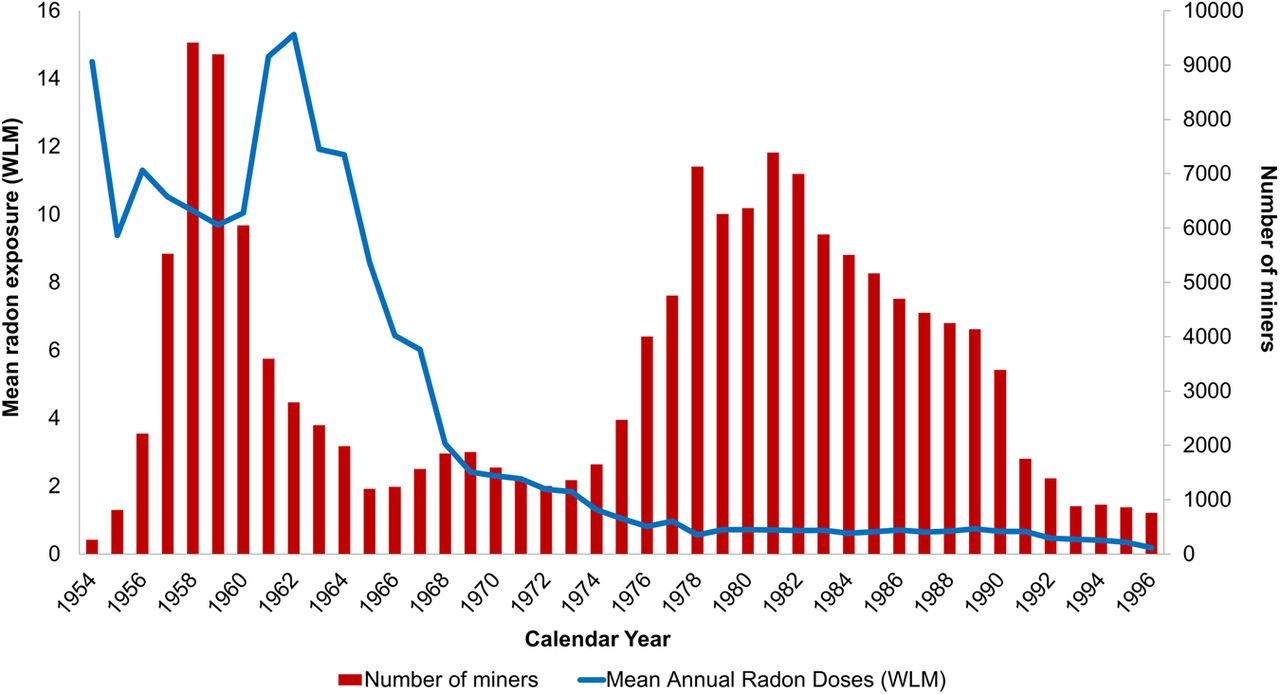
\includegraphics[width=\textwidth]{../assets/02-etiology/mortality_from_exposure_to_uranium.jpg}

    \small\textit{Cancer incidence and mortality from exposure to radon progeny among Ontario uranium
    miners. \cite{Navaranjan838}}
\end{center} 
\vspace{1em} 

\newpage

\begin{itemize}
    \item \textbf{Key Occupational Carcinogens:}
    \begin{itemize}
        \item \textit{Asbestos:} Strongly linked to lung cancer and mesothelioma; Risk escalates 
        sharply with cumulative exposure, even at low doses (no safe threshold). It causes direct 
        DNA damage via iron-generated reactive oxygen species (ROS) and chronic inflammation. 
        \cite{9498906}

        \item \textit{Silica dust (respirable crystalline silica):} Predominantly associated with 
        squamous cell and small cell carcinomas. Monotonic risk increase observed, with effects 
        detectable at cumulative exposures as low as 0.22 mg/m³-years. Accounts for 3\% of lung 
        cancer cases in industrialized nations, rising to 6\% \cite{CEBP2010} if all exposure levels 
        are considered.
    \end{itemize}

    \item \textbf{High-Risk Occupations:} Workers who are exposed, such as miners, shipyard 
    workers, insulators, textile plant workers, foundry workers, stonecutters, and ceramics 
    manufacturers, are at a significantly increased risk. 
\end{itemize}

% Safety practices: Hierarchical safety strategies to limit occupational cancer exposure.
Safety protocols to protect workers from key occupational carcinogens focus on minimizing exposure 
through a hierarchy of controls, combining elimination, engineering, administrative measures, and 
personal protective equipment (PPE). These protocols align with international occupational health 
guidelines and aim to keep exposure `As Low As Reasonably Achievable' (ALARA), effectively reducing 
the incidence of occupational cancers.
